\chapter{Data Understanding}

\textit{Credit Card Default} \`e un dataset la cui analisi si pone l\' obiettivo
di individuare i clienti a rischio di default, attraverso lo studio di quelli che sono i
movimenti in entrata ed uscita delle loro carte di credito.
Il periodo, a cui si riferiscono i dati in possesso, va da Aprile
a Settembre 2005 e la valuta di riferimento \`e il dollaro
taiwanese (NT\$). Il datasetet contiene 10.000 records descritti
da 24 colonne di attributi.

\section{Analisi degli attributi}

Di seguito (Tabella~\ref{tab1attributi}) vengono riportati
e descritti gli attributi raggruppandoli in base alla loro
tipologia e indicando per ciascuno di essi il loro dominio.

\begin{table}[H]
	\centering
	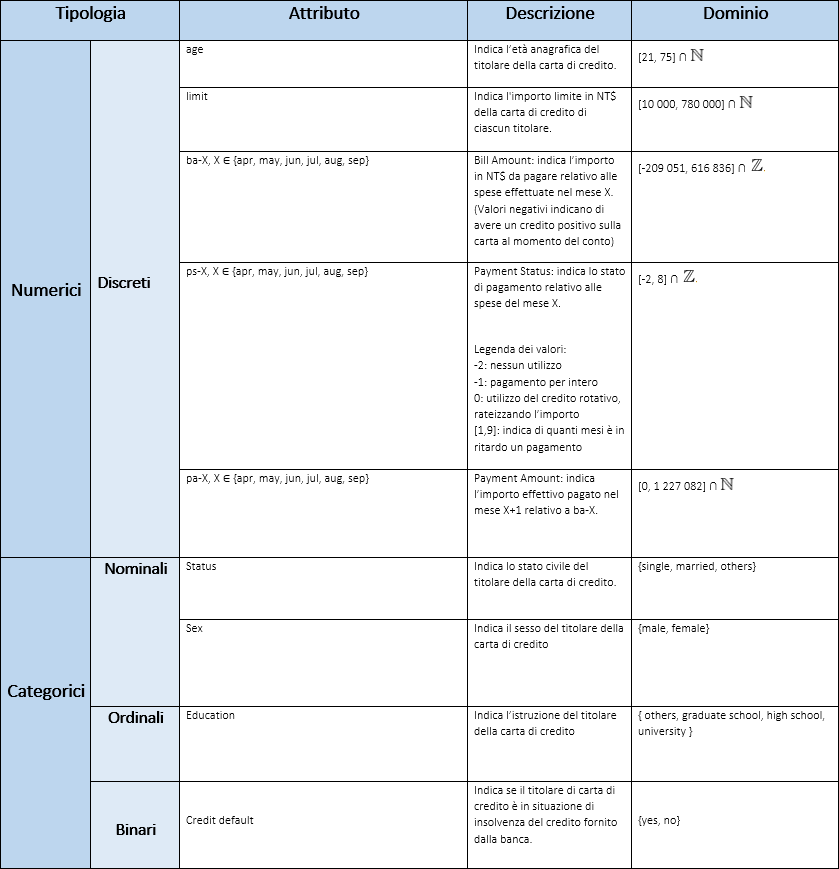
\includegraphics[width=12cm]{img/tabella1-attributi.png}
	\caption[LOF entry]{Attributi del dataset}
	\label{tab1attributi}
\end{table} 

\section{Analisi della qualit\`a dei dati}
\`E stata analizzata la qualit\`a dei dati all'interno del 
dataset fornito secondo i seguenti parametri:

\paragraph{Accuratezza Semantica}\mbox{}\\
Dal punto di vista semantico sono stati analizzati nello 
specifico gli attributi \texttt{payment amount},
\texttt{payment status} e \texttt{billing amount}.
L'attributo \texttt{payment amount} \`e stato confrontato
con l'attributo \texttt{billing amount} e \texttt{payment status}
per verificare a quale importo di pagamento si riferisse
il valore indicato \texttt{pa-\textit{X}}, ovvero
se \texttt{pa-apr}, per esempio, indicasse un pagamento
effettuato ad Aprile (quindi relativo al conto di Marzo) o
un pagamento del conto di Aprile (ndicato da \texttt{ba-apr})
e quindi effettuato a Maggio. Attraverso tale valutazione si
\`e concluso che il valore  \texttt{pa-\textit{X}} indica il
pagamento della cifra indicata dal \texttt{billing amount}
del mese precedente. Questo corrisponde alla realt\`a poich\`e
utilizzando una carta di credito, il pagamento effettuato in un
mese X \`e relativo all' importo da pagare del mese precedente.
Riprendendo l'esempio precedente, il pagamento relativo al conto
di Aprile (\texttt{ba-apr}) \`e indicato da \texttt{pa-may}. 
Da sottolineare la presenza di valori negativi nell'attributo
\texttt{ba-\textit{X}}, rappresentanti dal punto di vista semantico
una situazione di credito e non di debito nei confronti della banca.

\begin{figure}[H]
	\centering
	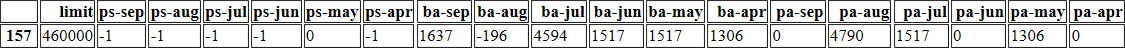
\includegraphics[width=\linewidth]{img/record-example.png}
	\caption[LOF entry]{
		un esempio di record che ha permesso
		facilmente di riconoscere il valore semantico degli attributi
		relativi alle transazioni monetarie. Si pu\`o notare grazie ai
		valori di \texttt{ps-\textit{X}}, come la cifra da pagare nel
		mese di Aprile, per esempio, sia equivalente alla cifra
		indicata nel pagamento di Maggio e lo stato di pagamento di
		aprile sia effettivamente -1, ovvero pagato completamente.
		Anche nei successivi mesi \`e possibile vedere un comportamento
		che corrisponde alla semantica degli attributi sopradescritta.
	}
	\label{record}
\end{figure}

Da sottolineare per\`o che per verificare il corretto
valore degli attributi  \texttt{pa-\textit{X}},
\texttt{ba-\textit{X}} e \texttt{ps-\textit{X}} sarebbe
necessario conoscere tutta la cronologia delle transazioni
di una specifica carta di credito cos\`i da poter calcolare
attraverso semplici operazioni aritmetiche i valori effettivi
di spese e pagamenti. Pertanto si \`e deciso di assumere come
corretti i dati considerando inoltre che essendo informazioni
raccolte da un istituto bancario non dovrebbero essere presenti
dati monetari errati. 

\paragraph{Gestione di Outliers e Missing Values}
Per la ricerca di outliers \`e stato prodotto per ciascun
attributo il relativo Boxplot, ma per la natura degli attributi
del dataset, i valori rappresentati come outliers nel boxplot,
non sono considerabili errati. Infatti per gli attributi numerici
che rappresentano somme di denaro (\texttt{pa-\textit{X}},
\texttt{ba-\textit{X}} e \texttt{limit}), abbiamo considerato
questi valori utili per le successive fasi di analisi sul
dataset. Lo stesso ragionamento vale per gli attributi 
\texttt{ps-\textit{X}}. Per quanto riguarda l'attributo
\texttt{age} invece, abbiamo considerato non utile escludere i record
per la loro bassa correlazione con qualsiasi altro attributo
del dataset. L'utilizzo dei boxplot ha sollevato una problematica
pi\`u facilmente osservabile da questi che non dal dataset, ovvero la presenza
dei Missing Values:

\subparagraph{attributi numerici}
 nessun attributo numerico relativo al plafond (\texttt{limit}), allo stato del pagamento (\texttt{ps-\textit{X}}) o alle transazioni della carta (\texttt{pa-\textit{X}}, \texttt{ba-\textit{X}}) presentano missing values.
 
\begin{wrapfigure}{r}{9cm}
\centering
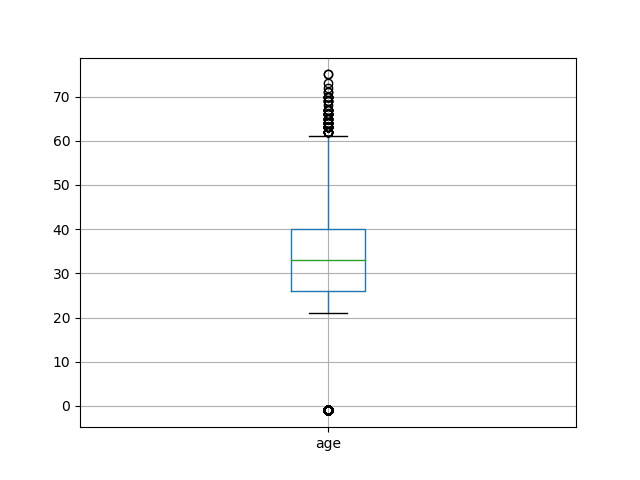
\includegraphics[width=8cm]{img/age-boxplot.png}
\caption{Boxplot del'attributo age}
\end{wrapfigure}

Un attributo numerico che presenta missing value \`e l'attributo \texttt{age}, infatti all'interno del dataset sono presenti per tale attributo molteplici valori -1, valore non coerente con un attributo che indichi l'et\`a anagrafica. \`E facilmente intuibile come tale valore indichi un valore mancante. Pertanto, tale valore \`e stato sostituito con la media dell'et\`a anagrafica dei record del dataset, ovviamente non tenendo conto dei valori -1. La media corrisponde a 35.4 che (per coerenza con il tipo di dato intero dell'et\`a) \`e stata troncata a 35 e settata in sostituzione del valore -1.\\\\
\subparagraph{attributi categorici}: ad eccezione di \texttt{credit\_default}, in ciascuno degli altri attributi categorici sono presenti missing values (nan), sostituiti dalla moda dell'attributo:
\begin{itemize}
\item \textbf{\texttt{sex}}: moda "female"
\item \textbf{\texttt{education}}: moda "university"
\item \textbf{\texttt{status}}: moda "single"
\end{itemize}

\section{Normalizzazione delle variabili}
Gli attributi \texttt{limit}, \texttt{ba-\textit{X}} e \texttt{pa-\textit{X}} rappresentando somme di denaro e pagamenti, hanno un ampio range di valori con massimo e minimo molto discostanti. Per utilizzare e visualizzare al meglio questi 3 attributi \`e stata utilizzata una normalizzazione \textbf{min-max}, trasformando il loro dominio in un range di valori continui [0,1].

\section{Distribuzione delle variabili e analisi statistiche}
\textbf{Attributi Numerici}\\
Per la visualizzazione della distribuzione di attributi numerici sono stati utilizzati degli istogrammi con curva gaussiana. Per gli attributi \texttt{limit},  \texttt{ba-\textit{X}}, \texttt{pa-\textit{X}}” e \texttt{age} si \`e scelto un numero di bins ottimale pari a 15 utilizzando la regola di Sturge, mentre per gli attributi  \texttt{ps-\textit{X}}, avendo un ristretto range di valori [-2, 8] si \`e utilizzato un numero di bins pari al numero di valori dell'attributo.

\begin{figure}[!htb]
\minipage{0.30\textwidth}
  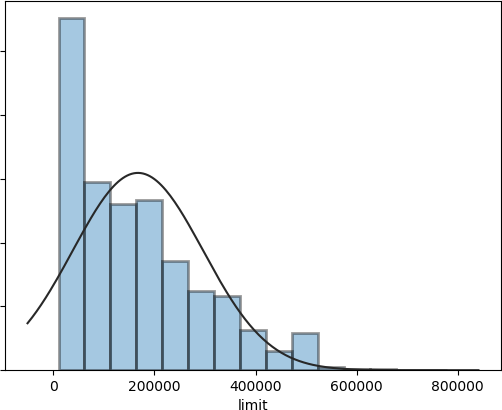
\includegraphics[width=\linewidth]{img/limit-distribution.png}
  \caption{Distribuzione attributo \texttt{limit}}\label{limit-dist}
\endminipage\hfill
\minipage{0.30\textwidth}
  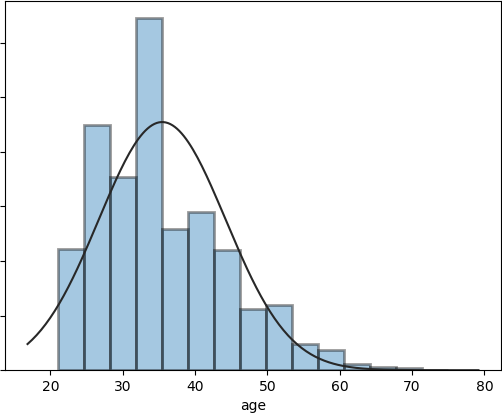
\includegraphics[width=\linewidth]{img/age-distribution.png}
 \caption{Distribuzione attributo \texttt{age}}\label{age-dist}
\endminipage\hfill
\minipage{0.35\textwidth}
  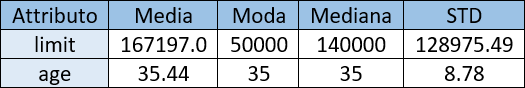
\includegraphics[width=\linewidth]{img/limit-age-stat.png}
\captionsetup{labelformat=empty}
\caption{Tabella 1.2: valori statistici \texttt{limit e age}}
	\label{limit-age-stat}
\endminipage
\end{figure}

Attraverso l'istogramma dell'attributo \texttt{limit} ( Figura~\ref{limit-dist}) \`e possibile vedere come il numero di clienti aventi quel determinato limite sia inversamente proporzionale al limmite stesso concesso dalla banca. Un comportamento dei dati che rispecchia la realt\`a, evidenziando come le persone pi\`u facoltose e con limiti di carta di credito pi\`u alte siano anche meno numerose. L'attributo \texttt{age} segue una distribuzione normale, infatti si pu\`o notare in Figura~\ref{age-dist} come il picco dell'istogramma coincida con la curva distribuzione, esattamente sul valore 35.

\begin{figure}[!htb]
\minipage{0.62\textwidth}
  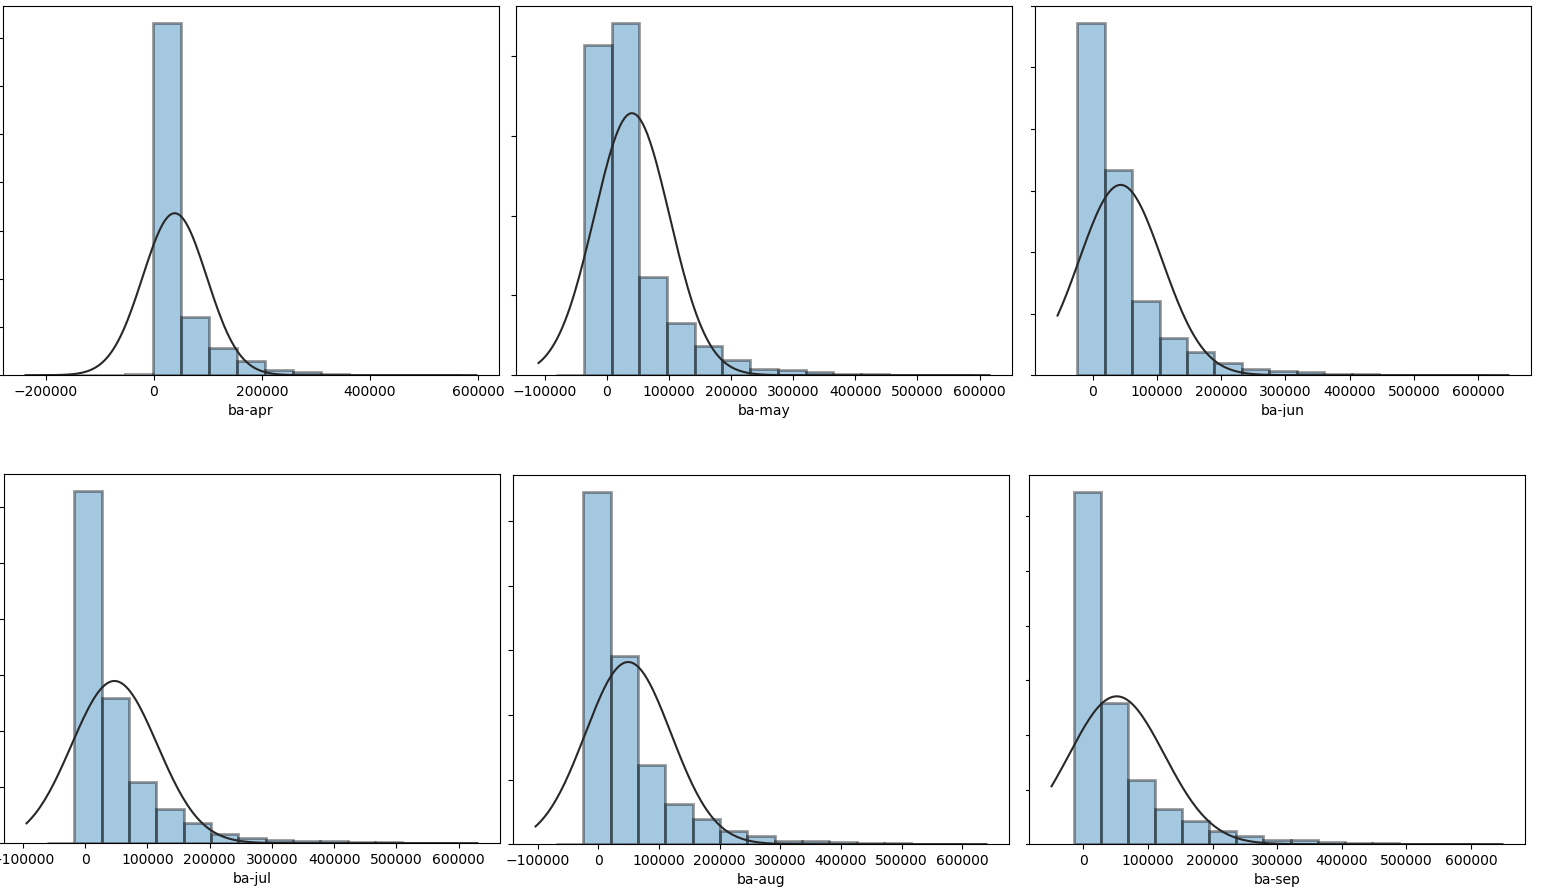
\includegraphics[width=\linewidth]{img/ba-distribution.png}
  \caption{Distribuzione attributo \texttt{ba-X}}\label{ba-dist}
\endminipage\hfill
\minipage{0.34\textwidth}
  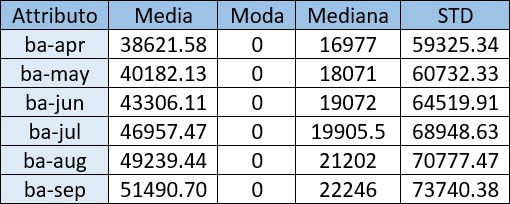
\includegraphics[width=\linewidth]{img/ba-stat.png}
\captionsetup{labelformat=empty}
\caption{Tabella 1.3: valori statistici \texttt{ba-\textit{X}}}
\label{ba-stat}
\endminipage\hfill
\end{figure}

\begin{figure}[!htb]
\minipage{0.62\textwidth}
  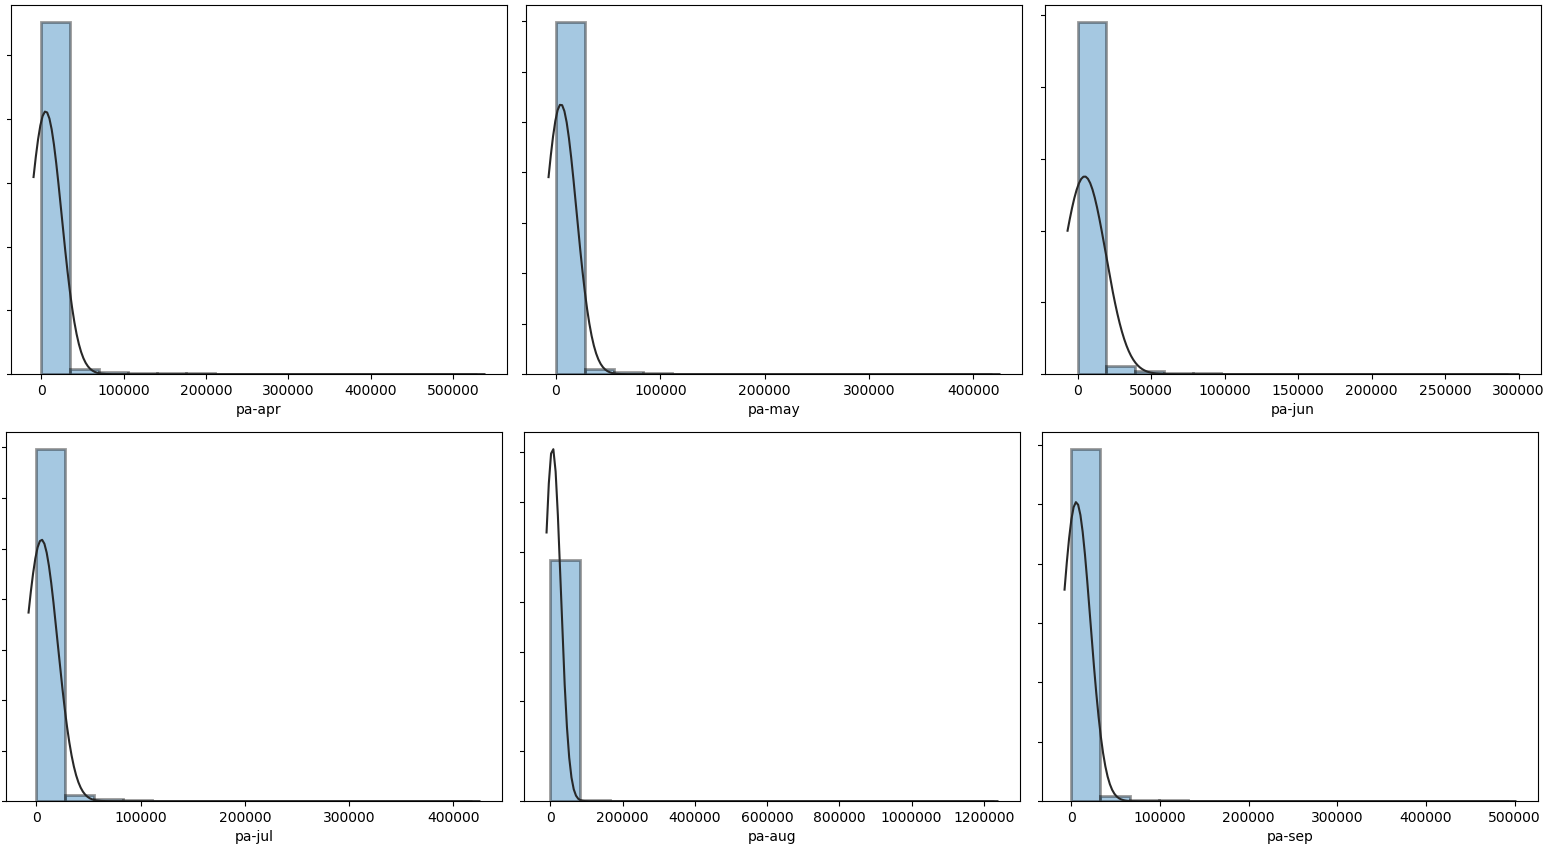
\includegraphics[width=\linewidth]{img/pa-distribution.png}
  \caption{Distribuzione attributo \texttt{pa-X}}\label{pa-dist}
\endminipage\hfill
\minipage{0.34\textwidth}
  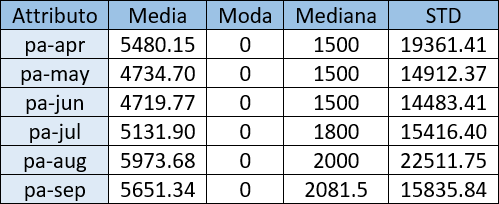
\includegraphics[width=\linewidth]{img/pa-stat.png}
\captionsetup{labelformat=empty}
\caption{Tabella 1.4: valori statistici \texttt{pa-\textit{X}}}
\label{pa-stat}
\endminipage\hfill
\end{figure}
\mbox{}\\
Per gli attributi \texttt{bill amount} e \texttt{payment amount} \`e possibile osservare come il numero di records aventi valori bassi sia molto alto. E' osservabile come il valore pi\`u ricorrente in entrambi i casi sia 0, ovvero che la maggior parte dei titolari di carta ogni mese non abbiano da pagare nessuna somma di denaro. Si pu\`o osservare come, nonostante siano presenti valori medi di \texttt{billing amount} piuttosto alti, per ogni mese il payment amount ha un valore medio di circa 5000. Osservando gli istogrammi in figura 1.10 e la Tabella 1.5 relativi ai payment status, si pu\`o giustificare la differenza di valori medi degli attributi \texttt{billing amount} e \texttt{payment amount} da un alto numero di titolari di carta che ricorrono al metodo di pagamento \textbf{revolving credit}, rappresentato dal valore 0 degli attributi \texttt{payment status}, valore pi\`u ricorrente.
Inoltre \`e da sottolineare come gli attributi \texttt{payment status} seguano a grandi linee una distribuzione normale, con picco sul valore 0.
\begin{figure}[!htb]
\minipage{0.62\textwidth}
  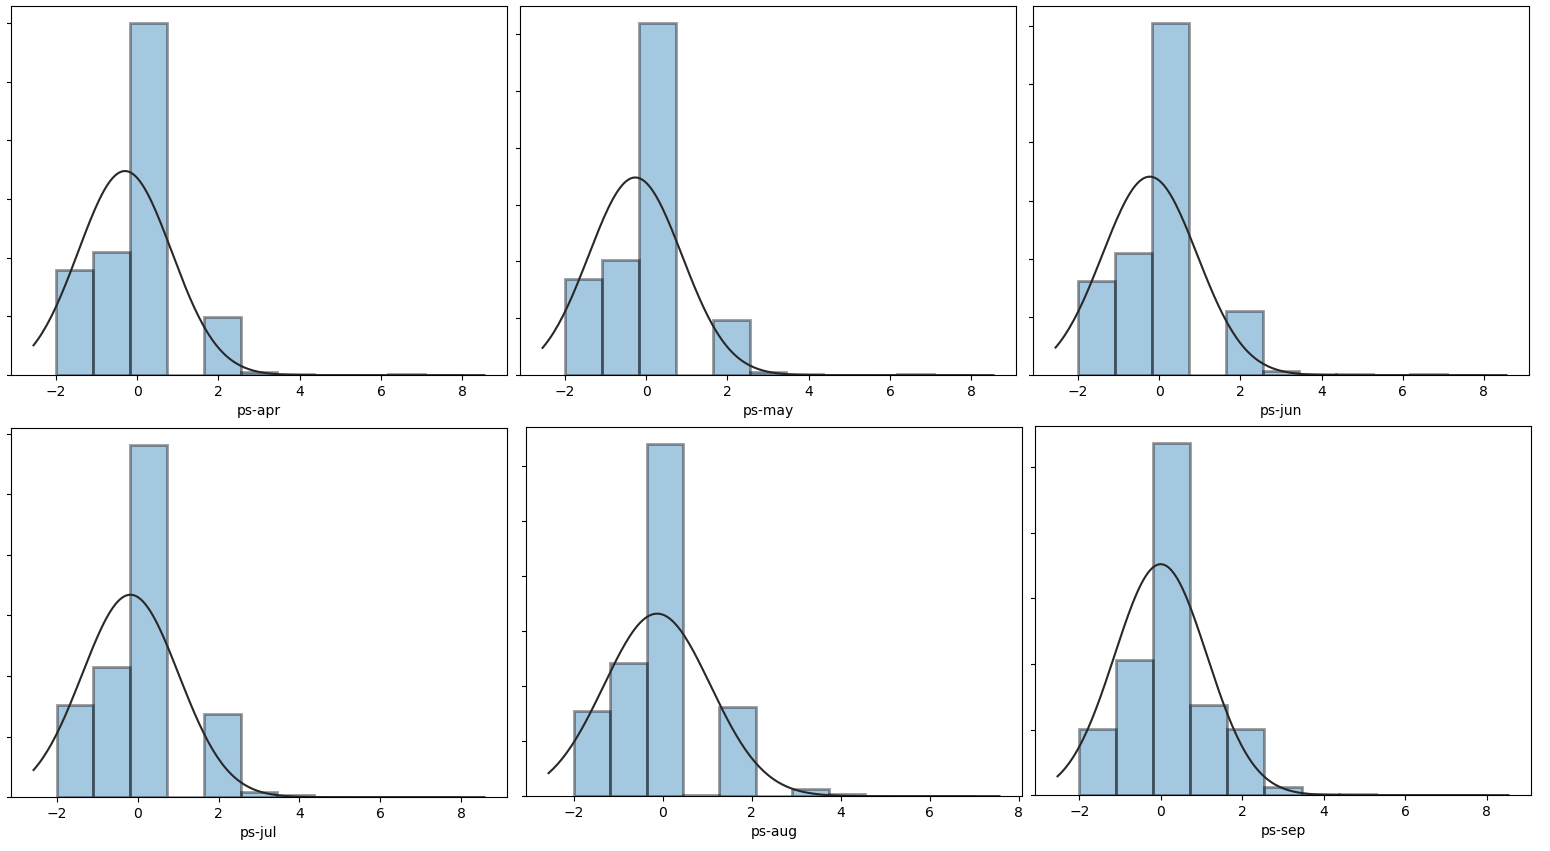
\includegraphics[width=\linewidth]{img/ps-distribution.png}
  \caption{Distribuzione attributo \texttt{ps-X}}\label{ps-dist}
\endminipage\hfill
\minipage{0.34\textwidth}
  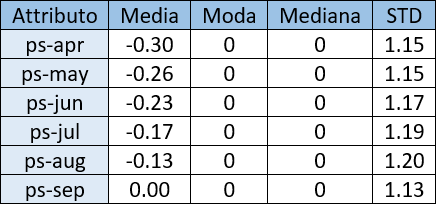
\includegraphics[width=\linewidth]{img/ps-stat.png}
\captionsetup{labelformat=empty}
\caption{Tabella 1.5: valori statistici \texttt{ps-\textit{X}}}
\label{ps-stat}
\endminipage\hfill
\end{figure}

\textbf{Attributi Categorici}
\begin{figure}[!htb]
\minipage{0.48\textwidth}
  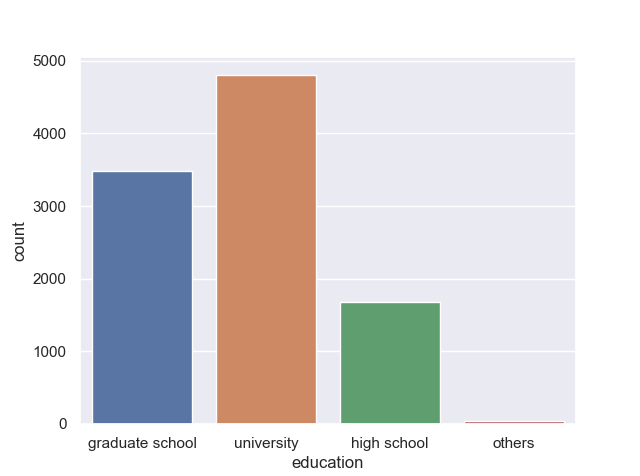
\includegraphics[width=\linewidth]{img/education-hist.png}
  \caption{Istogramma attributo \texttt{education}}\label{edu-dist}
\endminipage\hfill
\minipage{0.48\textwidth}
  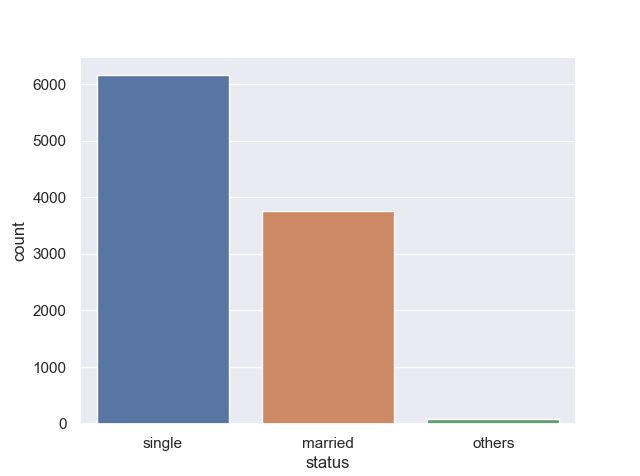
\includegraphics[width=\linewidth]{img/status-hist.png}
  \caption{Istogramma attributo \texttt{status}}\label{status-dist}
\endminipage\hfill
\end{figure}

Per gli attributi categorici \texttt{education} e \texttt{status}
sono stati generati gli istogrammi riportati in figura 1.12 e 1.13,
mentre per l'attributo \texttt{sex}, dato che presentava solamente
due valori, e l'attributo binario \texttt{credit\_default} si \`e
preferito l'utilizzo di grafici a torta.

\begin{figure}[H]
\minipage{0.48\textwidth}
  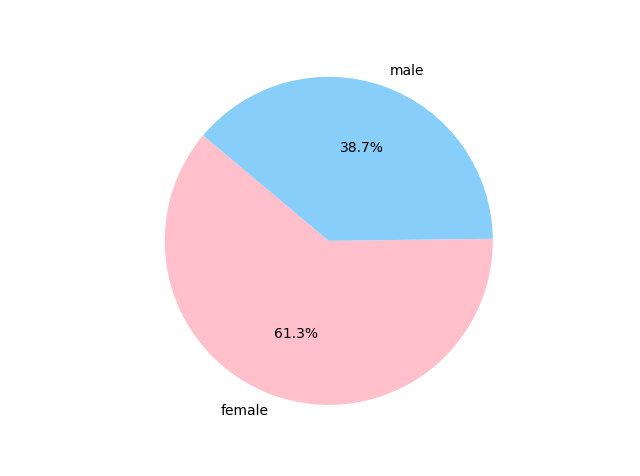
\includegraphics[width=\linewidth]{img/sex-dist.png}
  \caption{Istogramma attributo \texttt{sex}}\label{sex-dist}
\endminipage\hfill
\minipage{0.48\textwidth}
  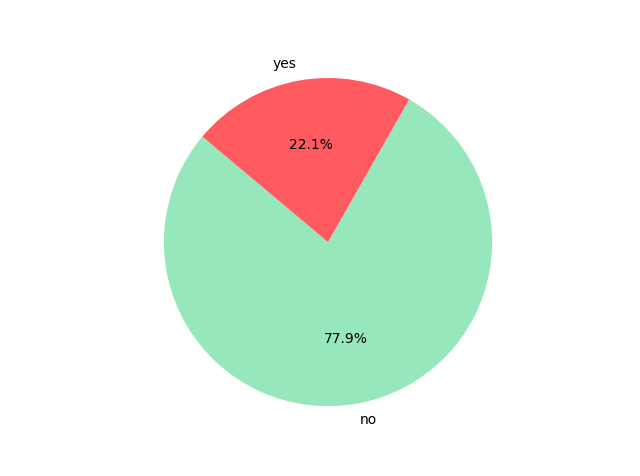
\includegraphics[width=\linewidth]{img/default-dist.png}
  \caption{Istogramma attributo \texttt{credit\_default}}\label{default-dist}
\endminipage\hfill
\end{figure}

\section{Correlazione tra variabili}
L'analisi della correlazione \`e stata fatta escludendo
gli attributi categorici e binari. Con riferimento alla 
heatmap in figura ~\ref{heatmap}, le correlazioni significative
sono, senza dubbio, quelle che occorrono tra i vari \texttt{payment status}
e \texttt{billing amount} di ogni mese, con tendenza decrescente per mesi
temporalmente pi\`u lontani. I valori alti di correlazione indicano una
tendenza nel mantenere il proprio comportamento nel tempo, sia esso positivo
(i.e, pagamenti in orario), sia esso
negativo nel caso dei \texttt{payment status}, o mantenere il proprio trend di spesa
nel caso dei \texttt{billing amount}.
Questo logicamente \`e del tutto normale in quanto se un individuo comincia a ritardare
i pagamenti (equivalente ad alzare il valore dell'attributo), \`e pi\`u facile che
i ritardi avvengano anche nei mesi successivi.
Mentre per il trend di spesa, dipende dallo stile di vita della persona.

\begin{figure}[h]
\centering
  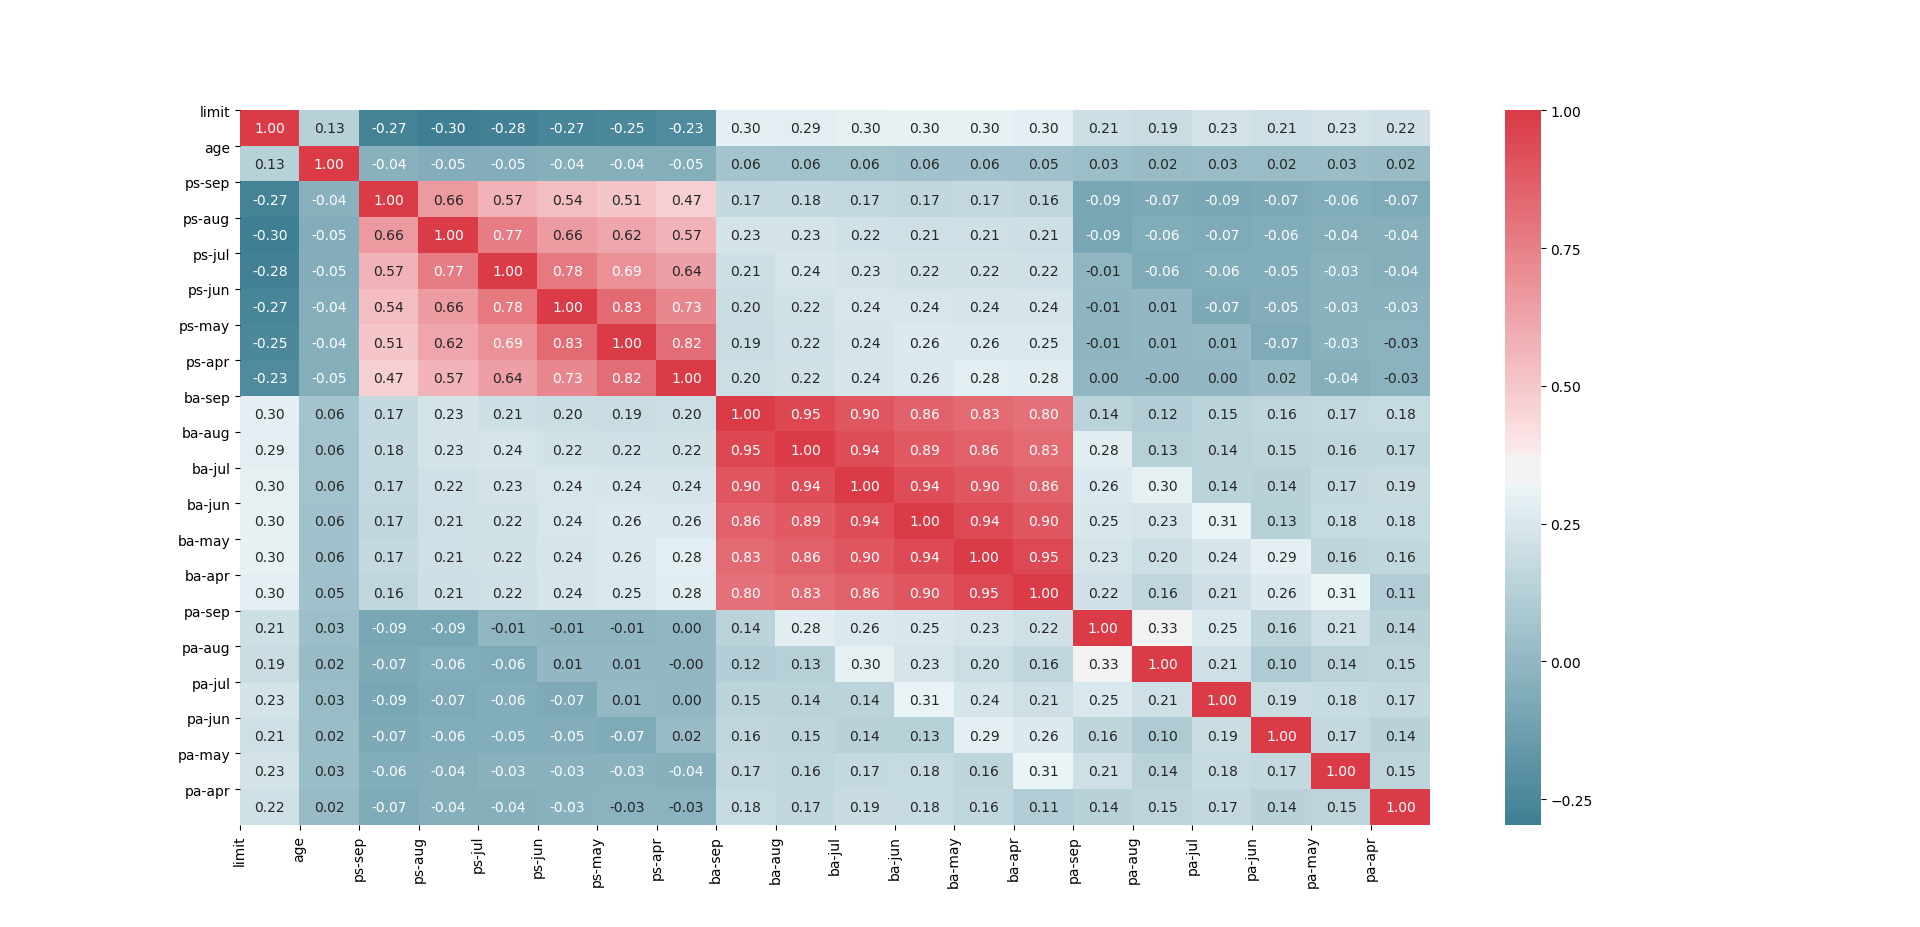
\includegraphics[width=.7\linewidth]{img/heatmap.png}
  \caption{Heatmap delle correlazioni tra attributi}
  \label{heatmap}
\end{figure}
